\documentclass[12pt,a4paper]{article}

\renewcommand*\contentsname{Sadržaj}
\renewcommand{\figurename}{Slika}

\usepackage[margin=0.85in]{geometry}
\usepackage{graphicx}
\usepackage{float}
\usepackage{listings}

% Default fixed font does not support bold face
\DeclareFixedFont{\ttb}{T1}{txtt}{bx}{n}{12} % for bold
\DeclareFixedFont{\ttm}{T1}{txtt}{m}{n}{12}  % for normal

% Custom colors
\usepackage{color}
\definecolor{deepblue}{rgb}{0,0,0.5}
\definecolor{deepred}{rgb}{0.6,0,0}
\definecolor{deepgreen}{rgb}{0,0.5,0}

% Python style for highlighting
\newcommand\pythonstyle{\lstset{
language=Python,
basicstyle=\ttm,
otherkeywords={self},             % Add keywords here
keywordstyle=\ttb\color{deepblue},
emph={MyClass,__init__},          % Custom highlighting
emphstyle=\ttb\color{deepred},    % Custom highlighting style
stringstyle=\color{deepgreen},
frame=tb,                         % Any extra options here
showstringspaces=false            % 
}}


% Python environment
\lstnewenvironment{python}[1][]
{
\pythonstyle
\lstset{#1}
}
{}

% Python for external files
\newcommand\pythonexternal[2][]{{
\pythonstyle
\lstinputlisting[#1]{#2}}}

% Python for inline
\newcommand\pythoninline[1]{{\pythonstyle\lstinline!#1!}}

% DODANO:
\renewcommand{\arraystretch}{1.5}
\begin{document}

\begin{titlepage}
	\centering
	{\scshape Univerzitet u Sarajevu \par}
	{\scshape Elektrotehnički Fakultet \par}
	\vspace{1cm}
	{\Large\scshape Prepoznavanje Oblika i Obrada Slike\par}
	\vspace{1.5cm}
	{\huge\bfseries Projektni Zadatak br. 2\par}
	\vspace{2cm}
	\Large Studenti: \par
	{\Large\itshape \textsc{Muftić} Belma, 1423/17260\par}
	{\Large\itshape \textsc{Lemeš} Lamija, 1474/17070\par}
	{\Large\itshape \textsc{Krupalija} Ehlimana, 1431/17461\par}
	\vfill
	Odgovorni asistent:\par
	MoE \textsc{Sumejja Porča}
	\vfill
	{\large December, 2018\par}
\end{titlepage}

\pagenumbering{gobble}

\tableofcontents

\newpage

\pagenumbering{arabic}
\setcounter{page}{1}

\section{Izbor modela za prepoznavanje}

Postoji šest najčešće korištenih klasifikacijskih modela (što je prikazano na Slici 1.):

\begin{enumerate}

\item SGD (\textit{Stohastic Gradient Descent}) klasifikacija;
\item \textit{Kernel Approximation} klasifikacija;
\item Linearna SVC (\textit{Support Vector Classification});
\item SVC (\textit{Support Vector Classification});
\item KNN (\textit{K-Nearest Neighbors}) klasifikacija;
\item \textit{Naive Bayes} klasifikacija.

\end{enumerate}

\begin{figure}[H]

\center
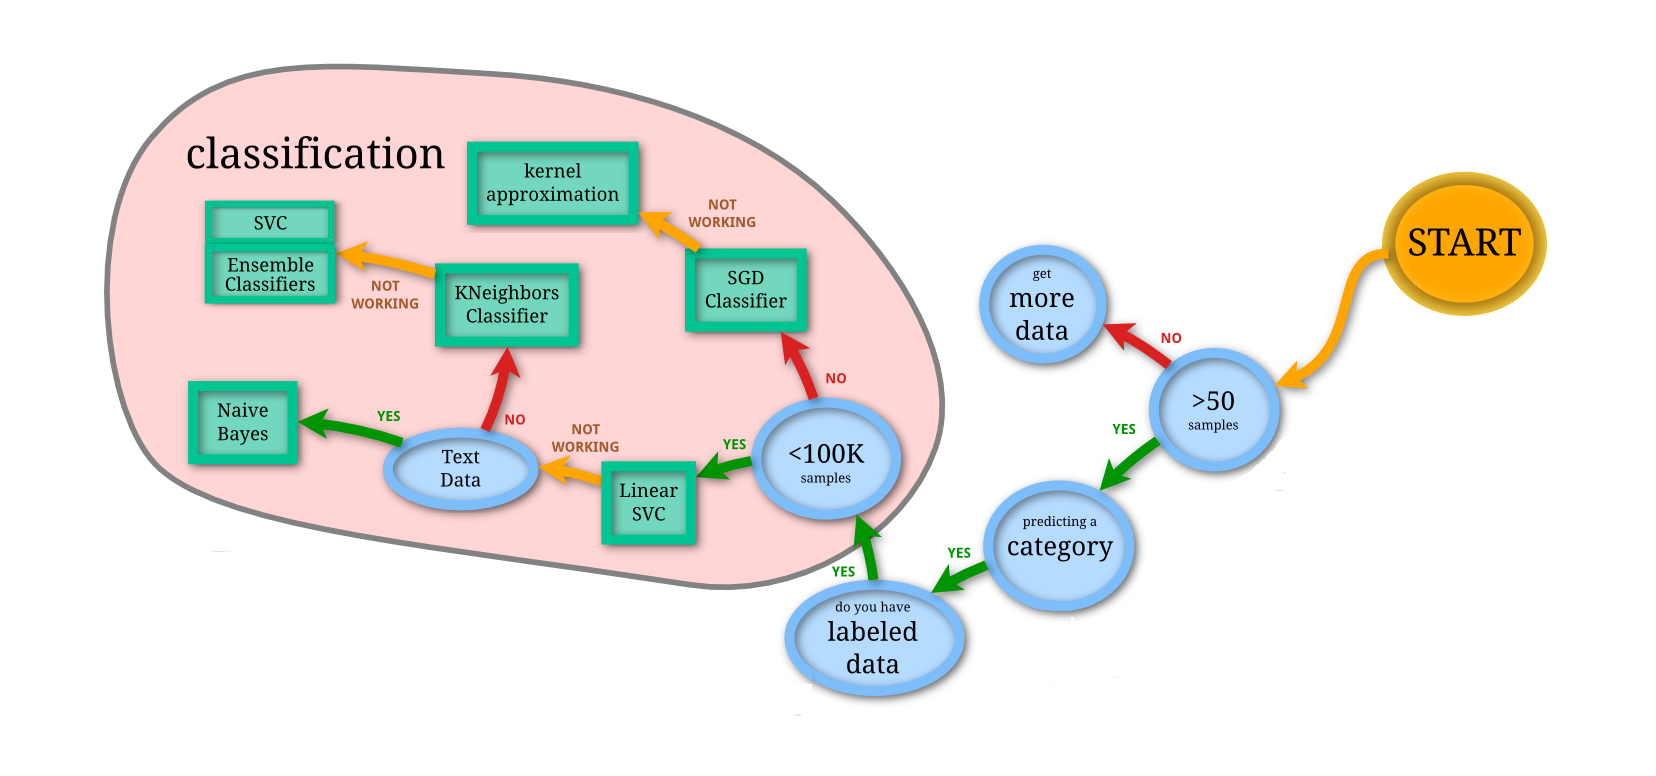
\includegraphics[scale=0.35]{slikaModeli.png}
\caption{Klasifikacijski modeli i vršenje njihovog odabira}
	
\end{figure}

Budući da \textit{dataset} ima manje od 100,000 slika, te postoje tekstualni podaci o različitim kategorijama i ROI, koristiti će se \textbf{\textit{Naive Bayes}} klasifikacijski model.

\newpage

\section{Izbor i kreiranje deskriptora}

Odabran je \textbf{\textit{HuMoments}} deskriptor, kako on opisuje oblik željenog objekta, a prepoznavanje ćelije se oslanja prvenstveno na njen oblik. U svrhu toga je kreirana skripta  \texttt{maskiranje.py} koja izloira samu ćeliju (dakle bez pozadine), jer se \textit{HuMoments} oslanja na analizu slika sa jednim kanalom.\\
~\\
Maskiranje je zasnovano na izdvajanju piksela koji spadaju u određeni rang vrijednosti, nakon čega se radi otvaranje da bi se uklonili ''zalutali'' pikseli, te se radi i dilatacija da bi se uključile i granice ćelije koje prethodno nisu bile u zadatom rasponu. Nakon maskiranja je pozvana funkcija \texttt{HuMoments} koja vraća niz brojeva koji opisuju oblik prethodno dobivene binarne slike. Nakon normalizacije niza, vrijednosti se zapisuju u CSV datoteku, te ako su u pitanju \textit{Train} slike, upisuje se i kojoj klasi slike pripadaju.\\
~\\
Navedene funkcionalnosti implementirane su na sljedeći način:\\

\pythonexternal{deskriptori.py}

\newpage

\section{Izbor metoda poboljšanja}

\subsection{Poboljšavanje kontrasta}

Od tri implementirane metode, najbolje rezultate pokazala je metoda \textbf{linearnog razvlačenja kontrasta}. Metoda aritmetičkih operacija previše je narušila strukturu slike, dok metoda \textit{gamma} korekcije nije izvršila dovoljnu modifikaciju kontrasta. Iz ovog razloga metoda linearnog razvlačenja kontrasta koristiti će se za poboljšavanje slika prije njihove dalje obrade.

\begin{figure}[H]

\center
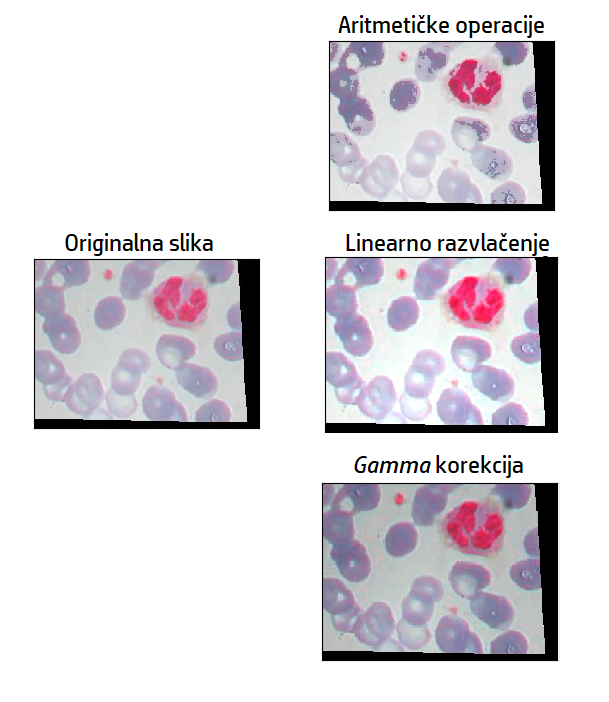
\includegraphics[scale=0.9]{slikaKontrast.png}
\caption{Rezultati korištenja različitih metoda za poboljšavanje kontrasta}
	
\end{figure}

\newpage

\subsection{Poboljšavanje osvjetljenja}

Od tri implementirane metode, najbolje rezultate pokazala je metoda \textbf{linearnih transformacija}. Metoda aritmetičkih operacija nije izvršila dovoljnu promjenu osvjetljenja, dok je metoda manipulacije HSV slikom izvršile preveliko povećanje osvjetljenja, te će se iz ovog razloga metoda linearnih transformacija koristiti za poboljšavanje slika prije njihove dalje obrade.

\begin{figure}[H]

\center
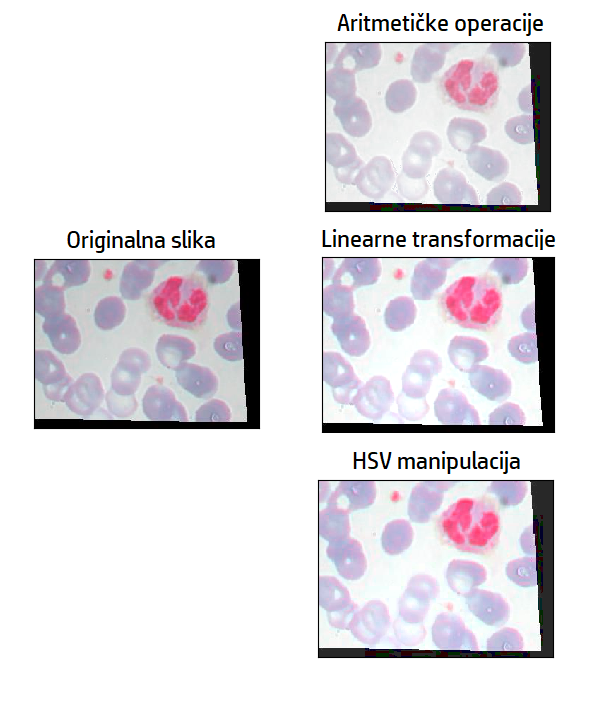
\includegraphics[scale=0.9]{slikaOsvjetljenje.png}
\caption{Rezultati korištenja različitih metoda za poboljšavanje osvjetljenja}
	
\end{figure}

\newpage

\subsection{Ujednačavanje histograma}

Od tri implementirane metode, najbolje rezultate pokazala je metoda \textbf{CLAHE}. Metoda raspodjele vjerovatnoća previše je degradirala strukturu slike (pri čemu su neke ćelije potpuno nestale sa slike, što je nedopustivo), dok je metoda \texttt{equalizeHist} degradirala strukturu slike u pogledu boje. Iz ovog razloga metoda CLAHE koristiti će se za poboljšavanje slika prije njihove dalje obrade.

\begin{figure}[H]

\center
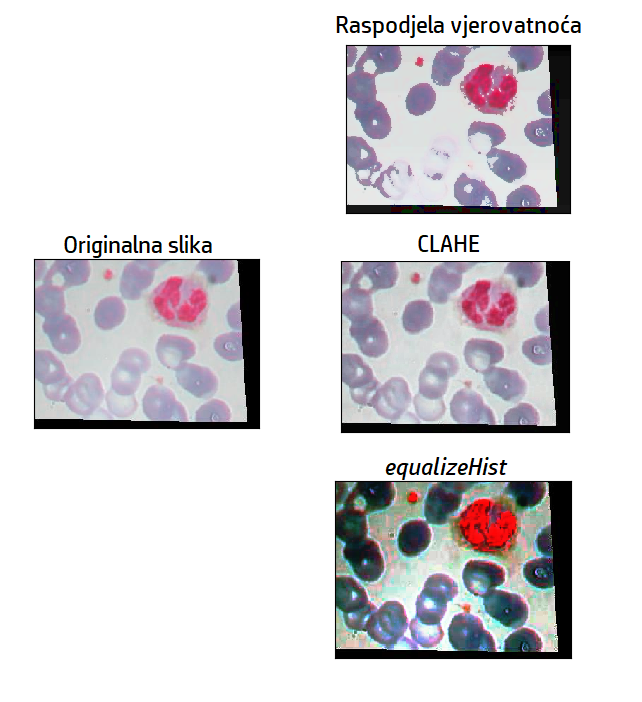
\includegraphics[scale=0.9]{slikaHistogram.png}
\caption{Rezultati korištenja različitih metoda za ujednačavanje histograma}
	
\end{figure}

\newpage

\section{Testiranje modela}

Kreirani deskriptori koriste se za treniranje i testiranje modela, pri čemu veoma važan aspekt predstavlja varijabla \texttt{confusionMatrix}, koja sadrži sve relevantne informacije o performansama modela. Na Slici 5. vidljivo je da je tačnost modela oko \textbf{76 \%}, te da najveću specifičnost pokazuje \textbf{klasa 1}, dok najveću senzitivnost pokazuje \textbf{klasa 2}. Najmanje vrijednosti specifičnosti i senzitivnosti ima \textbf{klasa 3}.

\begin{figure}[H]

\center
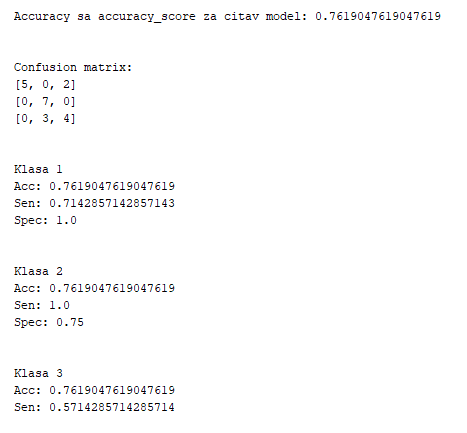
\includegraphics[scale=0.9]{slikaTest.png}
\caption{Rezultati pokretanja modela za prepoznavanje}
	
\end{figure}

\newpage

\section{Poboljšavanje performansi modela za prepoznavanje}

\subsection{Izmjena parametara modela}

\subsection{Drukčija podjela podataka}

\subsection{Izbacivanje \textit{outlier}-a slika}

\end{document}